
\section{Überspannungsableiter}
Im Folgenden wird mit Hilfe des Simulationsprogramms FEMM das Modell eines Überspannungsableiters erstellt und das tangentiale Elektrische Feld $E_t$ entlang der Mittelachse des Ableiters unter verschiedenen Bedingungen ermittelt. \\ \\
Um das Modell zu erzeugen wurde eine OctaveFEMM Routine geschrieben, diese ist unter dem Namen \tt{Aufgabe6\_2a.m} im Anhang zu finden. Als Parameter nimmt sie den Außendurchmesser \tt{d} des Rings entgegen und dessen Höhe \tt{z}. Der Parameter \tt{meshnet} bestimmt die Größe der zum Meshen benutzen Dreiecke. Es ist zu erwähnen, dass Kanten des unteren Mast und Teile der Antenne nicht modelliert werden, da sie beim Meshen nicht berücksichtigt werden sollen. Setz man dort die Materialproperty \tt{<No Mesh>}, um zu verhindern, dass diese gemesht werden, so endet das Programm mit einer Fehlermeldung.\\ \\
In Abbildung \ref{fig:Alle} ist der Überspannungsableiter sowie das entstehende Potenzial im Raum zu sehen. Die Randbedingungen werden für die rechte und die obere Begrenzung des Spannungsableiters gesetzt. Abb. \ref{fig:KeinRand} zeigt die Entwicklung des Potenzial, wenn keine Randbedingungen gesetzt wurden. Abb. \ref{fig:0VRand} hingegen zeigt das Potenzial, wenn am Rand die Bedingung von \SI{0}{\volt} gesetzt wird. Am oberen Mast, sowie an allen damit verbundenen leitenden PEC-Gebieten und am feldsteuernden Ring liegt ein Potenzial von \SI{471000}{\volt} an. Am Boden und am unteren Mast liegt das Potenzial \SI{0}{\volt} an. \\ \\
Da der Überspannungsableiter in der Realität nicht in einem geerdeten Kasten steht, ist es sinnvoller die Berechnung ohne explizite Randbedingungen durchzuführen. 
\newpage
\begin{figure}[h!]
	\centering
	\begin{subfigure}[h]{.28\textwidth}
		\centering
		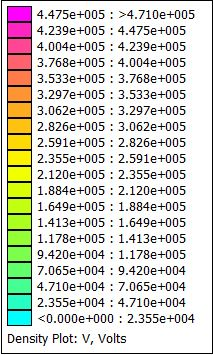
\includegraphics[width=\textwidth]{data/Skala}
		\caption{Skala}
		\label{fig:Skala}
	\end{subfigure}
	\begin{subfigure}[h]{.35\textwidth}
		\centering
		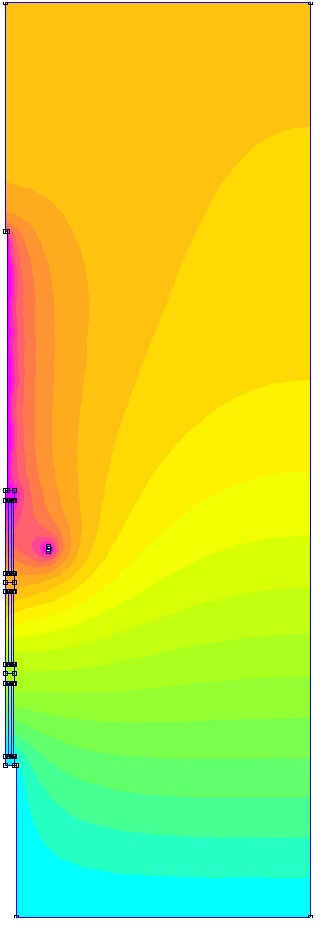
\includegraphics[width=\textwidth]{data/NoBoundary}
		\caption{Entwicklung des Potenzials ohne explizite Randbedingung}
		\label{fig:KeinRand}
		\vspace{-2pt}
	\end{subfigure}
	\begin{subfigure}[h]{.34\textwidth}
		\centering
		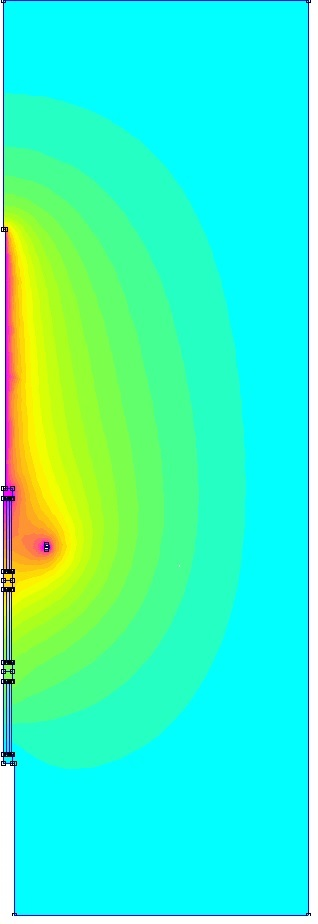
\includegraphics[width=\textwidth]{data/0VBoundary}
		\caption{Entwicklung des Potenzials mit Randbedingung \SI{0}{\volt}}
		\label{fig:0VRand}
	\end{subfigure}
	\caption{Überspannungsableiter mit unterschiedlichen Randbedingungen}
	\label{fig:Alle}
\end{figure}
\newpage
Darüber hinaus wurde untersucht, wie sich das tangentiale Elektrische Feld entlang der Symmetrieachse entwickelt. Das Feld wurde nur in den Ableitersegmenten in der Höhe zwischen \SI{2000}{\milli\meter} und \SI{5480}{\milli\meter} berechnet. In Abbildung \ref{fig:Vgl} sind die Stärken der tangentialen Elektrischen Felder zu sehen. Der blaue Graph entsteht, wenn keine Randbedingungen vorgegeben werden, der rote bei der Randbedingung \SI{0}{\volt}. Es ist zu erkennen, dass das elektrische Feld bei der Randbedingung \SI{0}{\volt} mit zunehmender Höhe deutlich stärker wird, als das Feld ohne Randbedingungen. \\ \\

\begin{figure}[h]
	\centering
	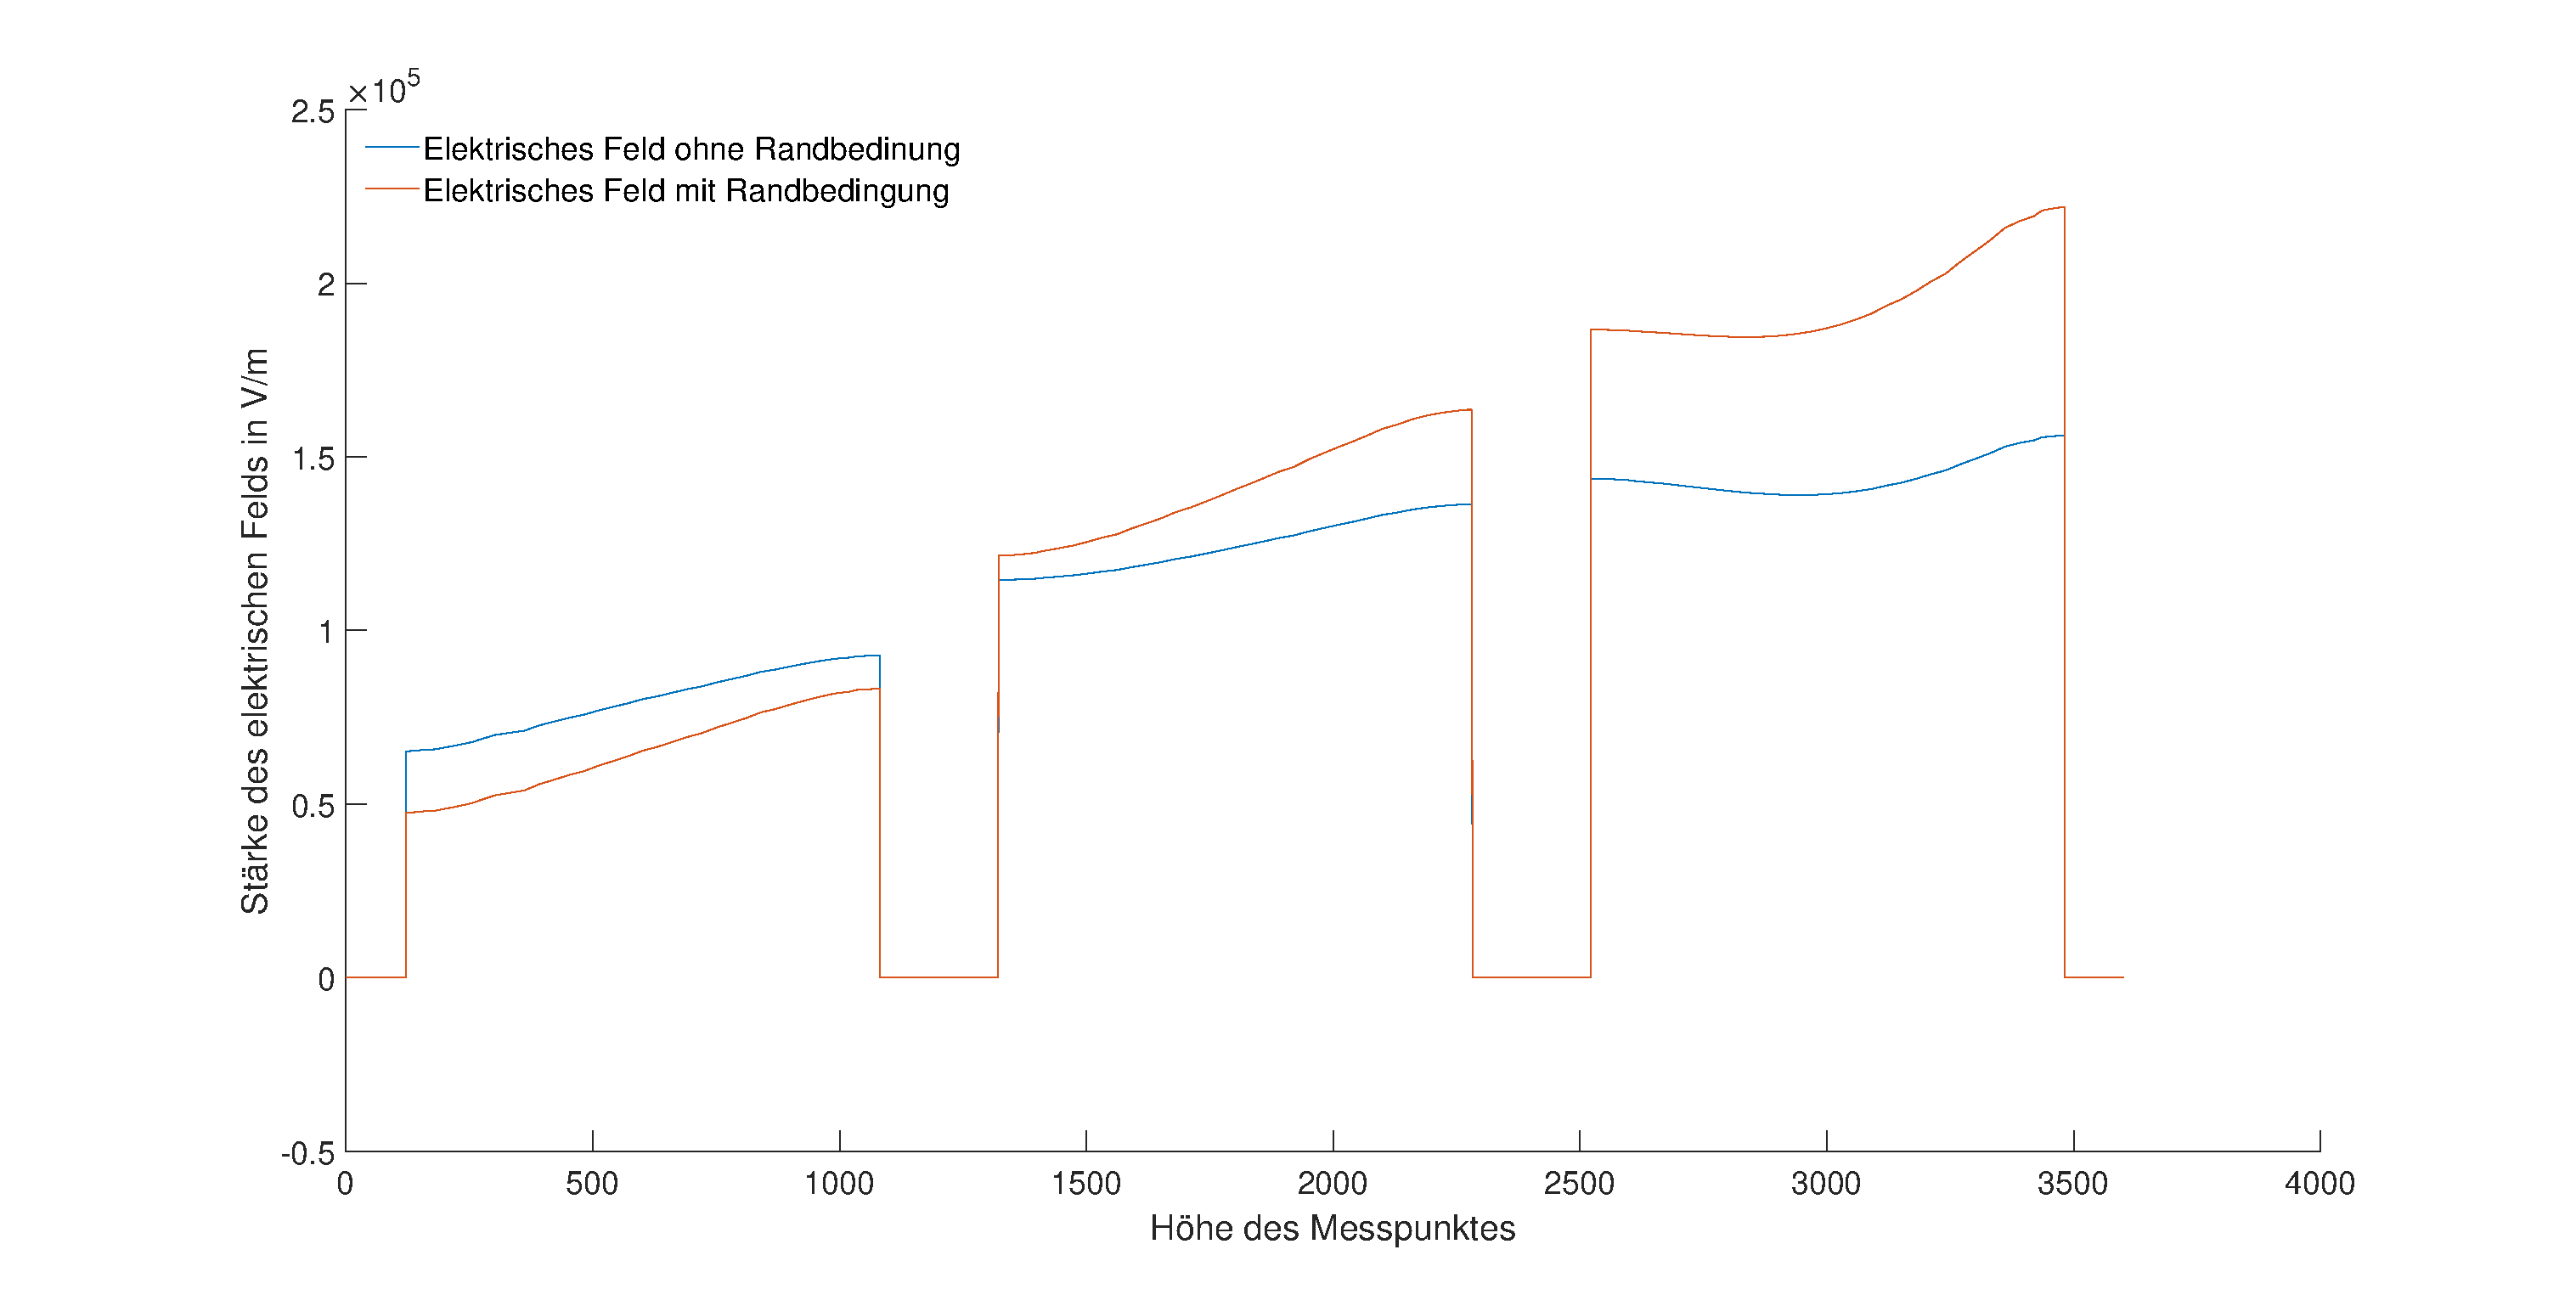
\includegraphics[width=\textwidth]{data/VergleichRandbedingung}
	\caption{Vergleich des tangentialen elektrischen Feldes bei unterschiedlichen Randbedingungen}
	\label{fig:Vgl}
\end{figure}


Zusätzlich gibt es bei FEMM die Möglichkeit das Gitter, das zum Meshen benutzt wird manuell einzustellen bzw. zu beeinflussen. Der Routine \tt{Aufgabe6\_2} wurden 120 unterschiedliche Netzgrößen von 10, bis minimal 0.8 übergeben und anschließend das tangentiale elektrische Feld berechnet. In Abbildung \ref{fig:Netz} sind diese Felder zu sehen. Bei der Verfeinerung des Gitters ließ sich kein Wert ermitteln, ab dem sich das Feld nicht mehr verändert. Beobachtet werden konnte, dass die maximale Netzgröße mit der FEMM arbeitet 10 und die minimale 0.8 beträgt. Der zum Vergleichen gewählte Messpunkt hat die Höhe \SI{4600}{\milli\meter}, auffällig ist, dass ab einer Netzgröße kleiner als eins (Messpunkt 100) die Rechenergebnis sehr stark variieren, wie in Abb. \ref{fig:NetzVGL} deutlich wird. \\ \\

\begin{figure}
	\centering
	\begin{subfigure}[h]{.8\textwidth}
		\centering
		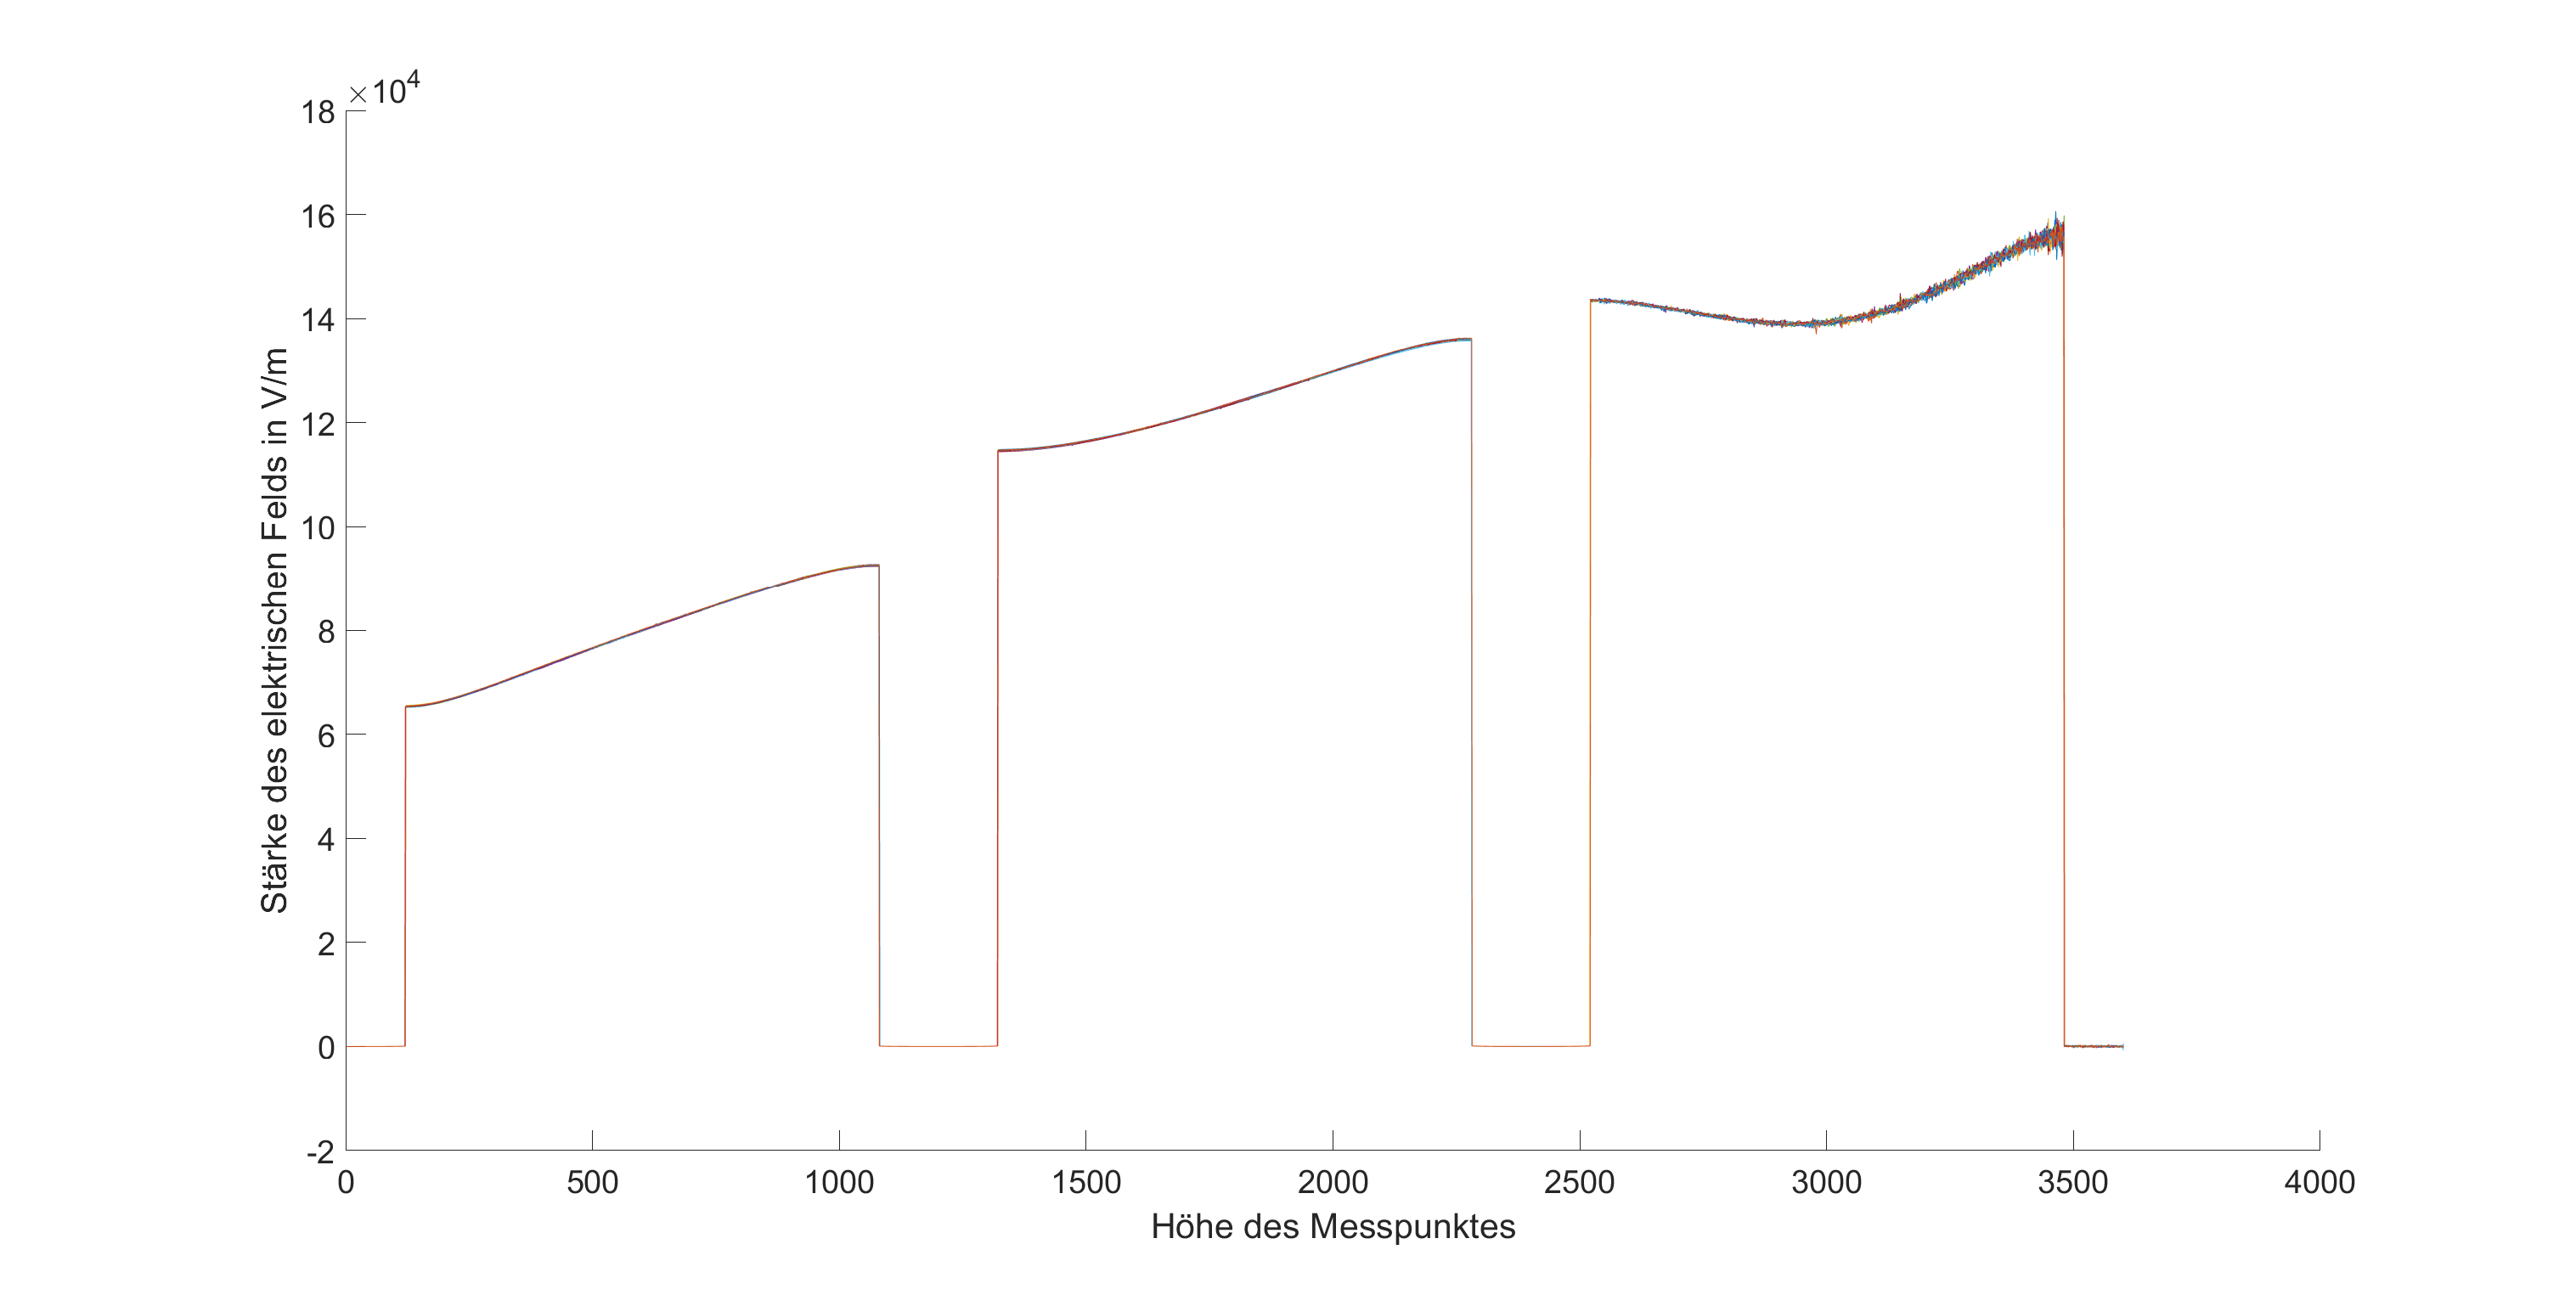
\includegraphics[width=\textwidth]{data/NetzVefeinerung}
		\vspace*{-28pt}
		\caption{Das tangentiale elektrische Feld mit unterschiedlichen Netzgrößen}
		\label{fig:Netz}
		
	\end{subfigure}
	
	\begin{subfigure}[h]{.8\textwidth}
		\centering
		\includegraphics[width=\textwidth]{data/NetzVefeinerungGroß}
		\caption{Detailausschnitt von \ref{fig:Netz}}
		\label{fig:NetzGroß}
	\end{subfigure}
	
	\begin{subfigure}[h]{.8\textwidth}
		\centering
		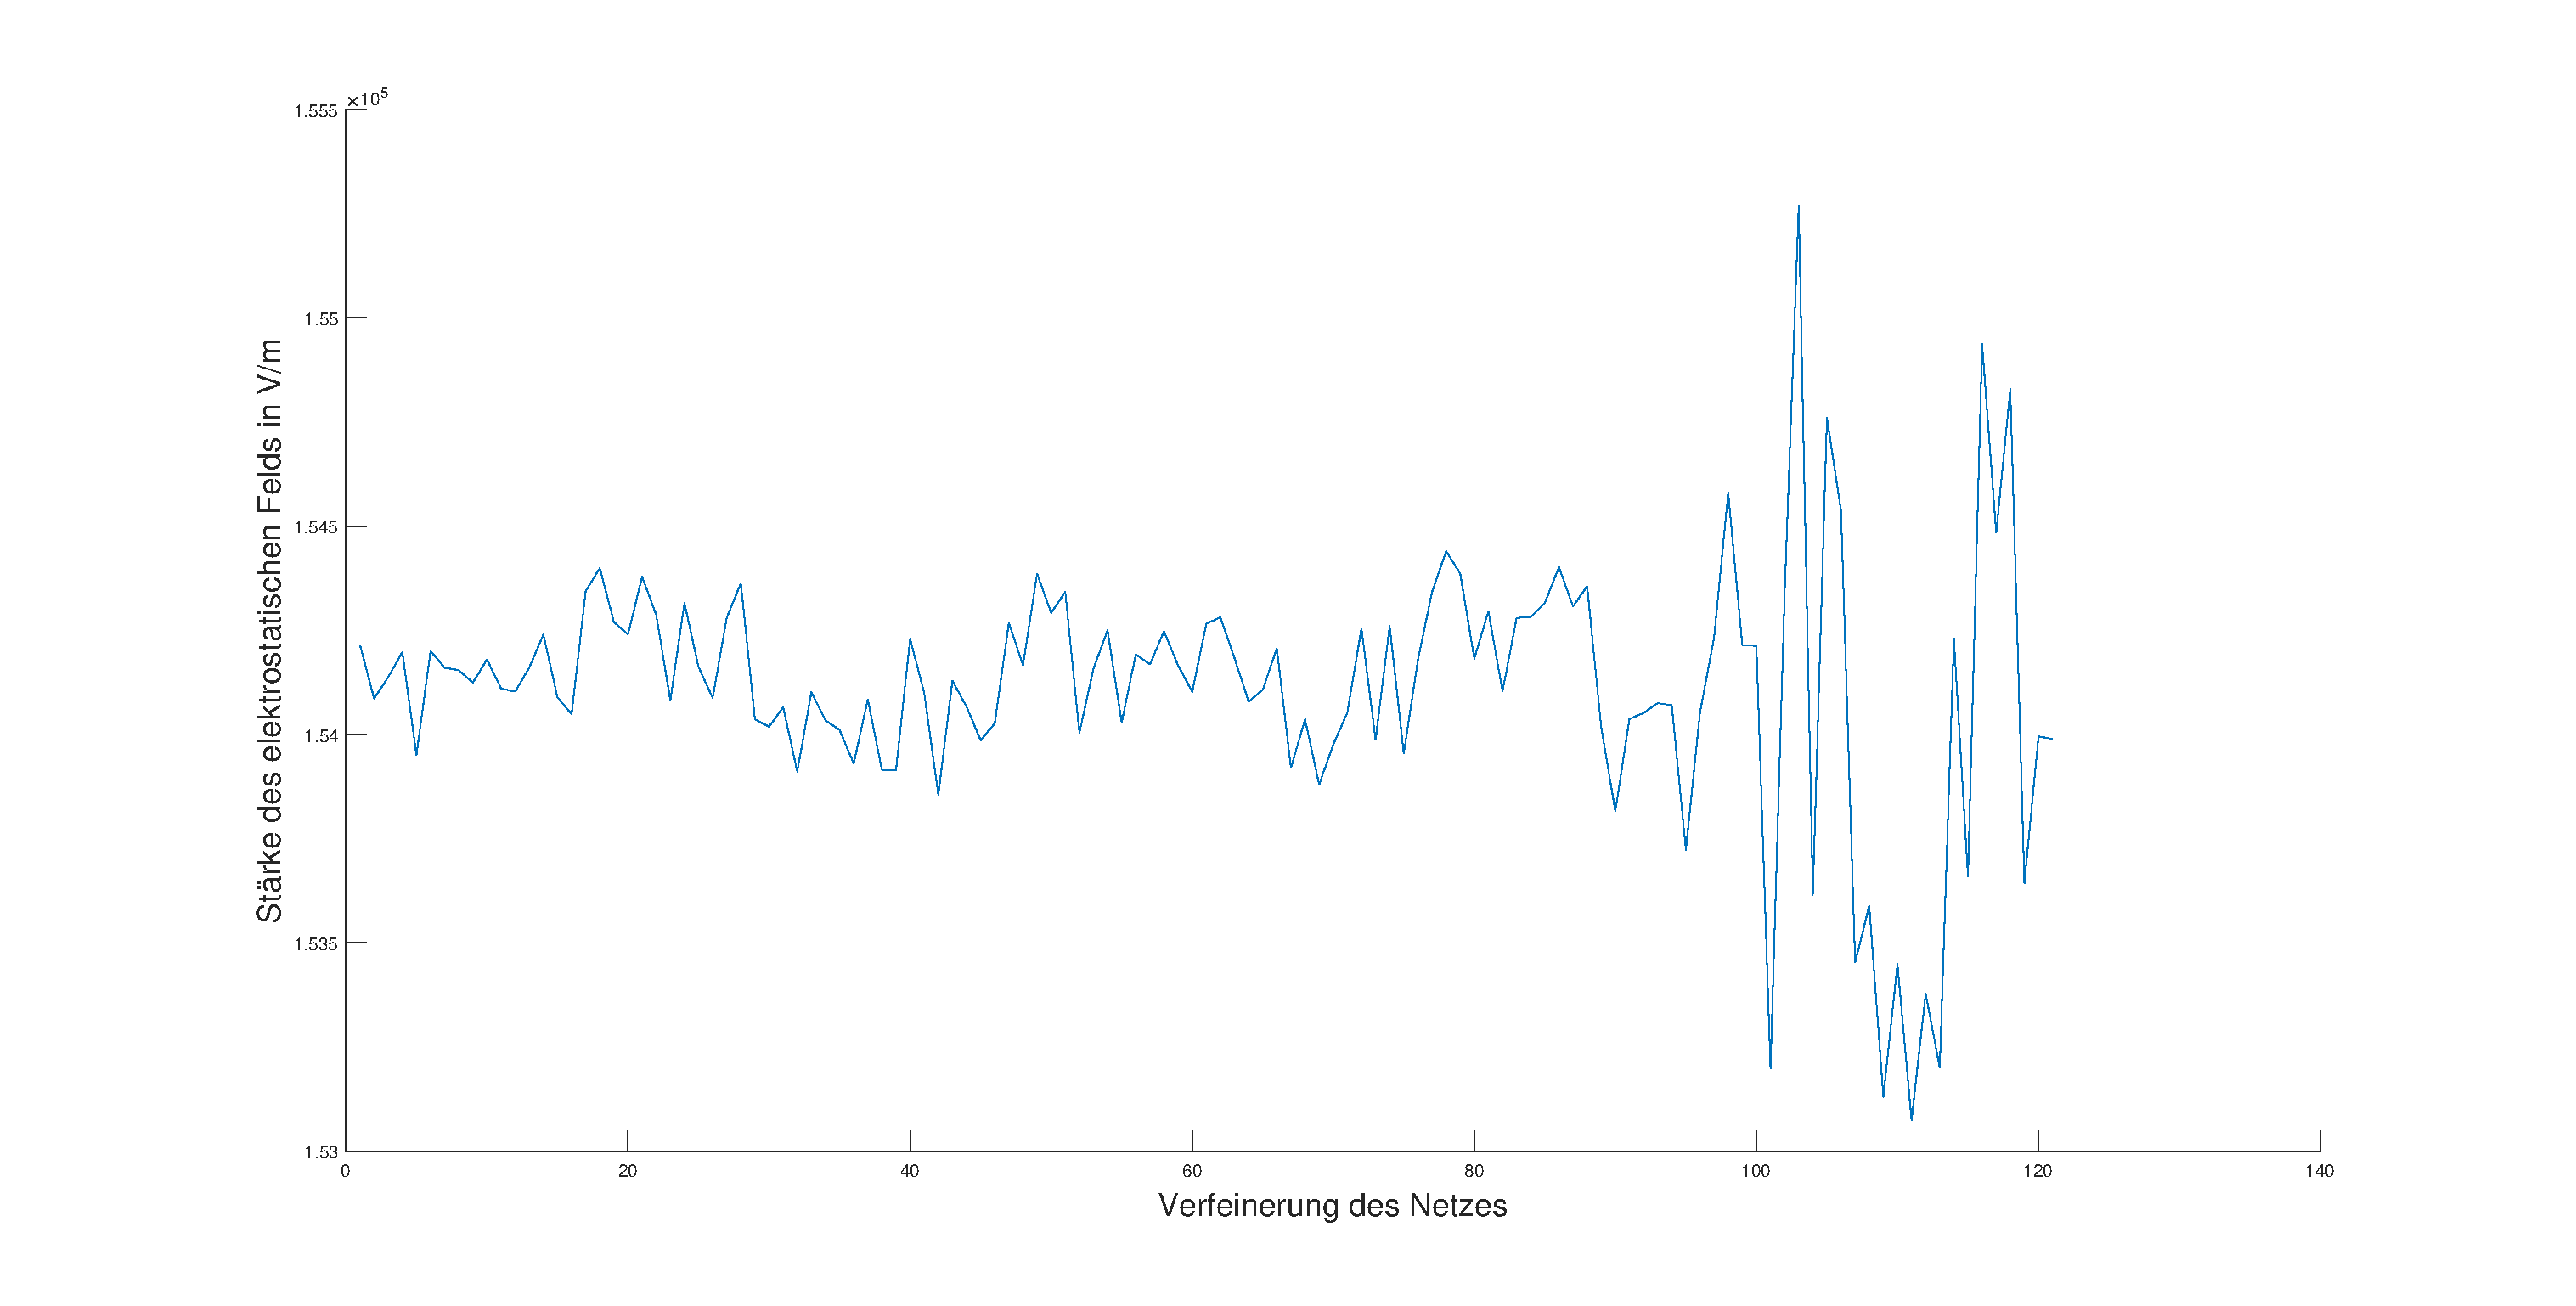
\includegraphics[width=\textwidth]{data/NetzVergleich}
		\caption{Stärke des elektrischen Feldes, abhängig von der gewählten Netzgröße}
		\label{fig:NetzVGL}
	\end{subfigure}
	\caption{Auswirkung der Verfeinerung des Gitters, das FEMM zum Meshen benutzt}
	
	%\label{fig:Alle}
\end{figure}

\newpage

Des Weiteren wurde die Auswirkung des feldsteuernden Rings auf das tangentiale elektrische Feld betrachtet. Zur Visualisierung des elektrischen Felds wurde der Octave Befehl \tt{surf} benutzt. Dadurch ist es möglich einen dreidimensionalen Plot zu erzeugen. Das elektrische Feld hängt dabei von der Höhe des Messpunktes und dem Außendurchmesser $d_a$ des Rings ab, dieser variiert zwischen \SI{600}{} und \SI{2000}{\milli\meter}. Dem  Modell wurden keine Randbedingungen vorgegeben. \\
Die tangentialen elektrischen Felder sind in der Abbildung \ref{fig:3DTang} zu sehen. Auffällig ist, dass bei steigendem Abstand zwischen dem Ring und dem Mast sich die elektrischen Felder unterschiedlich verändern. Das elektrische Feld in dem oberen und mittleren Ableitersegment nimmt ab, während es im untersten Segment ein stärkeres Feld entsteht.
\begin{figure}[h]
	\begin{subfigure}[h]{\textwidth}
		\centering
		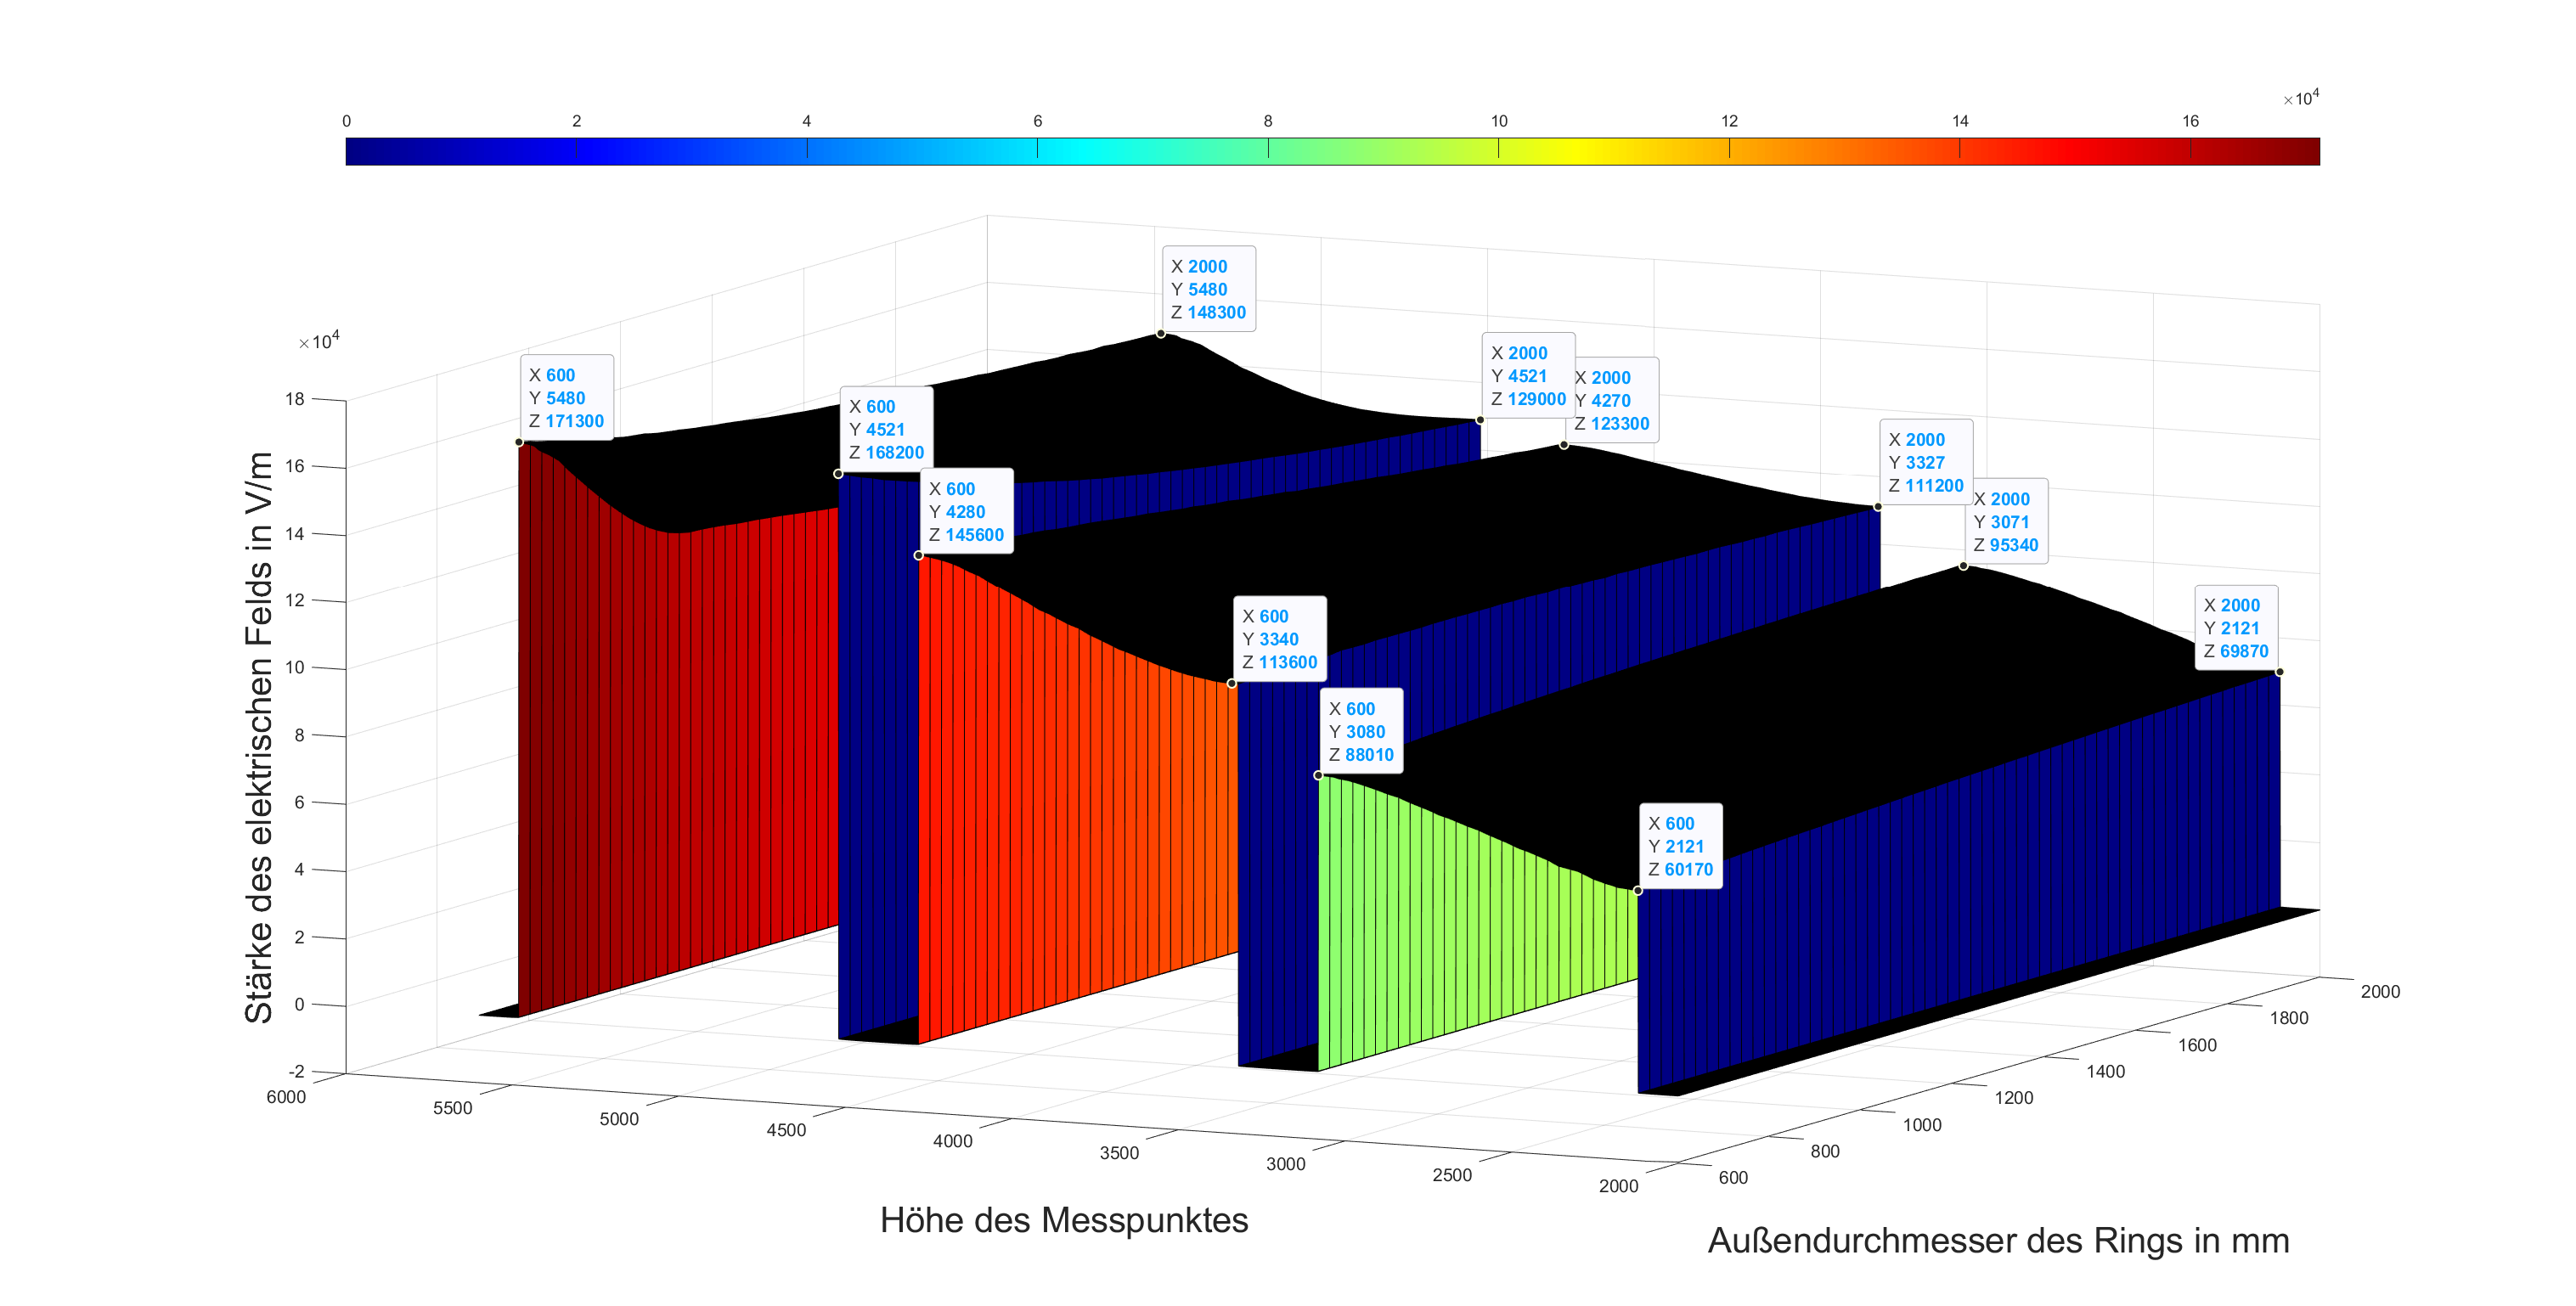
\includegraphics[width=\textwidth]{data/3DEtang}
	\end{subfigure}
	\begin{subfigure}[h]{\textwidth}
		\centering
		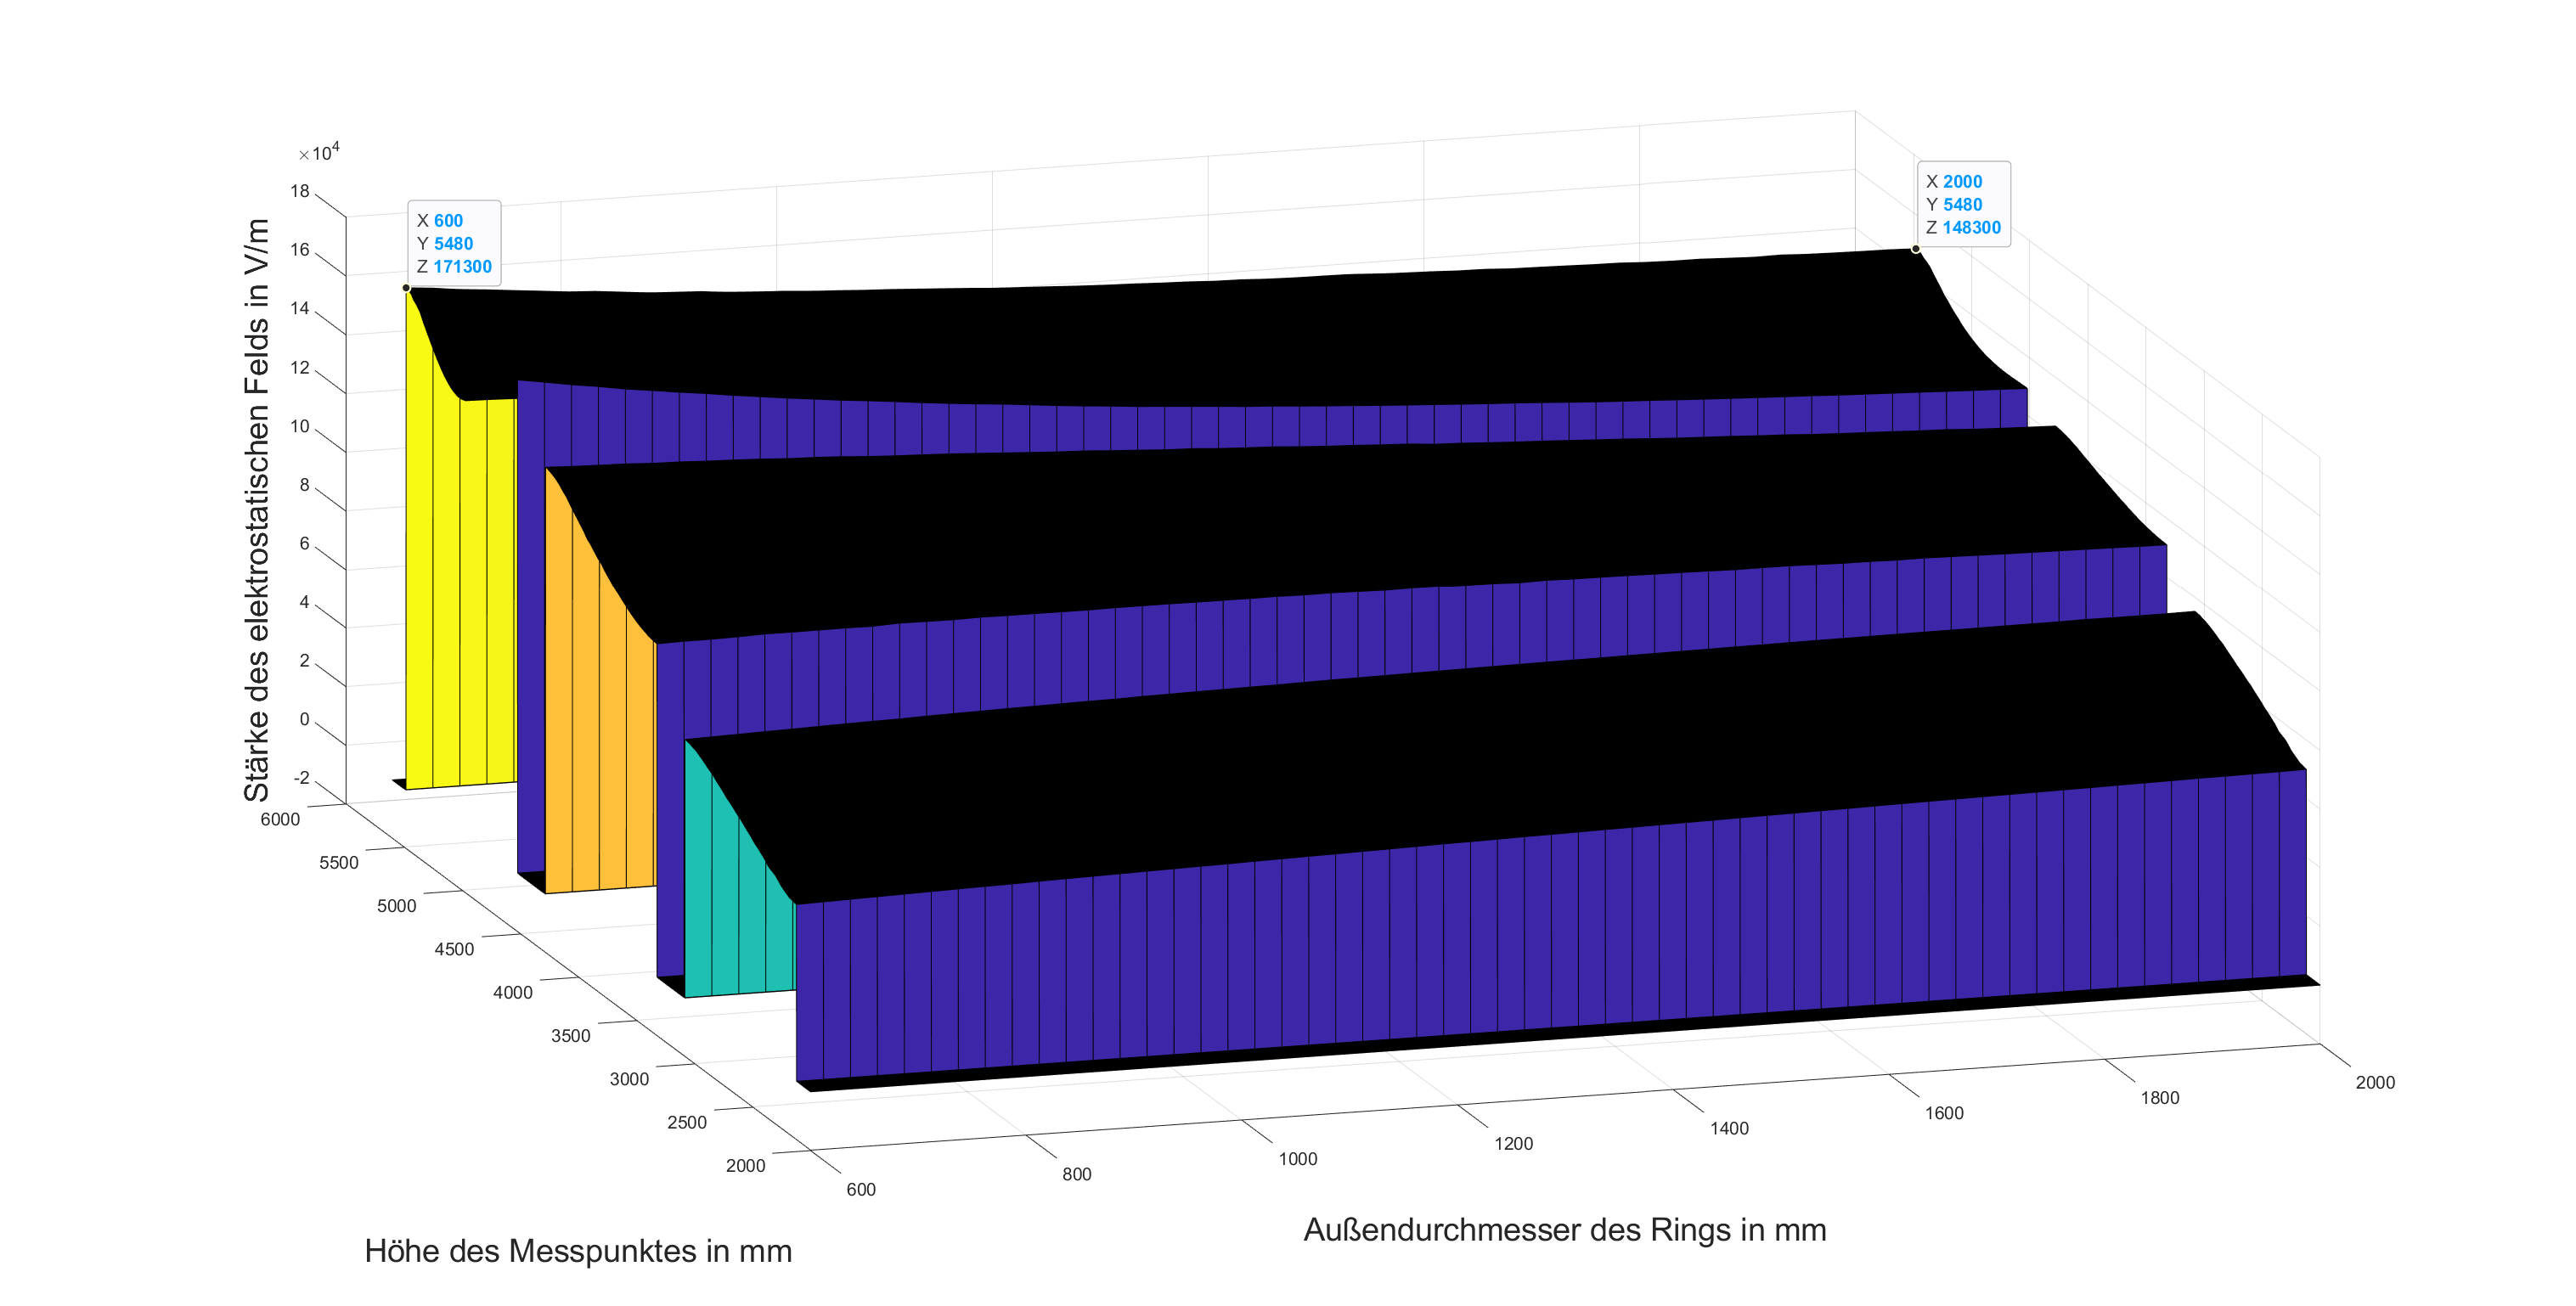
\includegraphics[width=\textwidth]{data/3DEtangVergleich}
	\end{subfigure}
\caption{Das tangentiale elektrische Feld in Abhängigkeit des Außendurchmesser des Rings und der Höhe des Messpunktes}
\label{fig:3DTang}
\end{figure}



